% Intended LaTeX compiler: pdflatex
\documentclass[10pt,a4paper,UTF8]{article}
\usepackage{zclorg}
\usepackage{tikztheorem}
\author{张朝龙}
\date{}
\title{练习:正交基}
\hypersetup{
 pdfauthor={张朝龙},
 pdftitle={练习:正交基},
 pdfkeywords={},
 pdfsubject={},
 pdfcreator={Emacs 25.0.50.1 (Org mode 9.0.6)},
 pdflang={English}}
\begin{document}

\maketitle
\tableofcontents
\titlepic{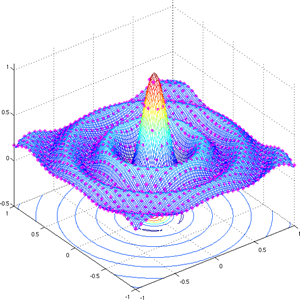
\includegraphics[scale=0.25]{../../img/sinc.PNG}}

\section{6.B.1}
\label{sec:org40dbcf4}


\begin{tikzproblem}
\begin{enumerate}
\item 设\(\theta\in \mathbf{R}\),证明\((\cos\theta,\sin\theta),(-\sin\theta,\cos\theta)\)和\((\cos\theta,\sin\theta),(\sin\theta,-\cos\theta)\)都是\(\mathbf{R}^{2}\)的规范正交基。
\item 证明\(\mathbf{R}^{2}\)的规范正交基一定是第一步中的二者之一。
\end{enumerate}
\end{tikzproblem}

\begin{tikzanswer}
对于第一步,我们只需要证明这两个向量组是规范正交向量组,然后因为其维度是2,而\(\mathbf{R}^{2}\)的维度也是\(2\)。很容易证明这两个向量组都是\(\mathbf{R}^{2}\)的规范正交基。

对于第二步我们假设\((u,v)\)是\(\mathbf{R}^{2}\)规范正交基的一个向量,则必有\(u^{2} + v^{2} = 1\),所以令\(u=\cos\theta\),\(v=\sin\theta\)。则与\((\cos\theta,\sin\theta)\)正交的向量有两种写法分别是\((\sin\theta,-\cos\theta)\)和\((-\sin\theta,\cos\theta)\).
\end{tikzanswer}
\section{6.B.2}
\label{sec:org40a3f30}


\begin{tikzproblem}
设\(e_{1},\ldots ,e_{m}\)是\(V\)的规范正交组。设\(v\in V\),证明:
\begin{equation}
\label{eq:2}
\| v \|^{2} = | \langle v,e_{1} \rangle  |^{2} + \ldots + | \langle v,e_{m} \rangle  |^{2}
\end{equation}
当且仅当\(v\in \mathrm{span}(e_{1},\ldots ,e_{m})\)
\end{tikzproblem}

\begin{tikzanswer}
这个问题的证明,首先我们证明当\(v\in \mathrm{span}(e_{1},\ldots ,e_{m})\)时,\(\| v \|^{2} = | \langle v,e_{1} \rangle  |^{2} + \ldots + | \langle v,e_{m} \rangle  |^{2}\) .
因为\(v\in \mathrm{span}(e_{1},\ldots ,e_{m})\),所以\(v\)在\(e_{1},\ldots ,e_{m}\)张开的空间中,这这个空间里,\(e_{1},\ldots ,e_{m}\)是规范正交基。所以\(v\)可以用\(e_{1},\ldots ,e_{m}\)和对应的坐标来表示,即:
\begin{equation}
\label{eq:3}
v = \langle v,e_{1} \rangle e_{1} + \ldots + \langle v,e_{m} \rangle e_{m}
\end{equation}
对上式使用勾股定理,则有:
\begin{equation}
\label{eq:4}
\| v \|^{2} = | \langle v,e_{1} \rangle  |^{2} + \ldots + | \langle v,e_{m} \rangle  |^{2}
\end{equation}

接下来我们证明第二步。假设\(\| v \|^{2} = | \langle v,e_{1} \rangle  |^{2} + \ldots + | \langle v,e_{m} \rangle  |^{2}\),我们要证明\(v\in \mathrm{span}(e_{1},\ldots ,e_{m})\)。

首先我们令:
\begin{equation}
\label{eq:5}
\xi = v - \langle v,e_{1} \rangle e_{1} + \ldots + \langle v,e_{m} \rangle e_{m}
\end{equation}
显然\(\xi\)与 \(e_{i},i=1,\ldots ,m\)正交,因为\(\langle \xi,e_{i} \rangle  = \langle v,e_{i} \rangle  - \langle v,e_{i} \rangle  =0\)
这意味着:
\begin{equation}
\label{eq:6}
\| v \|^{2} =  \| \xi \|^{2} + | \langle v,e_{1} \rangle  |^{2} + \ldots + | \langle v,e_{m} \rangle  |^{2}
\end{equation}
又因为\(\| v \|^{2} = | \langle v,e_{1} \rangle  |^{2} + \ldots + | \langle v,e_{m} \rangle  |^{2}\),所以\(\xi = 0\)。因此:\(v = \langle v,e_{1} \rangle e_{1} + \ldots + \langle v,e_{m} \rangle e_{m}\),即\(v\in \mathrm{span}(e_{1},\ldots ,e_{m})\)
\end{tikzanswer}
\section{6.B.3}
\label{sec:org5d44523}


\begin{tikzproblem}
设\(T\in \mathcal{L}(\mathbf{R}^{3})\),关于基\((1,0,0),(1,1,1),(1,1,2)\)具有上三角矩阵,求\(\mathbf{R}^{3}\)上一个规范正交基,使得\(T\)关于这个基具有上三角矩阵。
\end{tikzproblem}

\begin{tikzanswer}
根据舒尔定理,我们知道这个规范正交基存在。这个规范正交基通过对已经存在上三角矩阵的基的格拉姆施密特过程保证。因此求解这个规范正交基的过程是对\((1,0,0),(1,1,1),(1,1,2)\) 执行格拉姆施密特正交化的过程。
\end{tikzanswer}
\end{document}
